% =====================================================================
%  Energy Efficiency of LLM-Generated Code:
%  A Cross-Language and Cross-Platform Empirical Study
% ---------------------------------------------------------------------
%  Build:  latexmk -pdf main.tex      (or use LaTeX Workshop in VS Code)
%  Layout: IEEE conference format (two-column). IEEEtran.cls/.bst are
%          bundled in this folder (CTAN, v1.8b).
% =====================================================================
\documentclass[conference]{IEEEtran}

% --- Encoding & fonts -------------------------------------------------
\usepackage[T1]{fontenc}
\usepackage[utf8]{inputenc}
\usepackage{microtype}

% --- Math, tables, figures --------------------------------------------
\usepackage{amsmath,amssymb}
\usepackage{booktabs}
\usepackage{multirow}
\usepackage{graphicx}
\usepackage{placeins}  % \FloatBarrier before the references (G10)
\graphicspath{{figures/}}
\usepackage{xcolor}
\usepackage{enumitem}
\usepackage{fvextra}
\fvset{breaklines=true,breakanywhere=true}

% --- References -------------------------------------------------------
\usepackage{cite}
\usepackage[hidelinks]{hyperref}
\usepackage[capitalise,noabbrev]{cleveref}

% --- Working notes (set to [disable] for the final version) -----------
\setlength{\marginparwidth}{1.6cm}
\usepackage[colorinlistoftodos,textsize=scriptsize]{todonotes}
\newcommand{\TODO}[1]{\todo[inline,color=orange!25]{\textbf{TODO:} #1}}
\newcommand{\TBD}{\textcolor{red}{[TBD]}}

% --- Project-specific macros ------------------------------------------
\newcommand{\RQ}[1]{\textbf{RQ#1}}
\newcommand{\HYP}[1]{\textbf{H#1}}

% ---------------------------------------------------------------------
\title{Energy Efficiency of LLM-Generated Code:\\
       A Cross-Language and Cross-Platform Empirical Study}

\author{%
  \IEEEauthorblockN{Brisild Capani}
  \IEEEauthorblockA{DHBW Stuttgart\\
    \texttt{inf24039@lehre.dhbw-stuttgart.de}}
  \and
  \IEEEauthorblockN{Seyyid Bachri Oglou}
  \IEEEauthorblockA{DHBW Stuttgart\\
    \texttt{inf24071@lehre.dhbw-stuttgart.de}}
}

\begin{document}
\maketitle

\begin{abstract}
Evaluations of LLM-generated code focus on correctness rather than the energy the code
consumes when executed. We study energy efficiency along three factors: the generating LLM
(Claude, GPT, and Gemini via their official coding CLIs), the language (Python, Java,
C++), and the hardware platform. 630 programs for 14 tasks are checked for correctness and
measured under controlled conditions. \TODO{Final results.}
\end{abstract}

\begin{IEEEkeywords}
Large language models, code generation, energy efficiency, green software engineering,
empirical study
\end{IEEEkeywords}

\section{Introduction}
\label{sec:introduction}

Code-generation benchmarks measure correctness, not the energy generated code consumes.
Prior studies find that this energy varies between
models~\cite{solovyeva2025powerhungry,islam2025evaluating,apsan2026whereare}, but each
varies only some factors: several languages without platform
interactions~\cite{solovyeva2025powerhungry,rekhi2026prompting}, or several platforms for
Python only~\cite{apsan2026whereare}. Whether ``model~A generates more efficient code than
model~B'' holds beyond one language and machine is untested~\cite{masthanali2026slr}.

In a full factorial experiment, three LLMs, accessed through their official coding CLIs,
solve 14 tasks in Python, Java, and C++, and every correct program is measured on an
x86 laptop and an Arm Mac. We ask which LLM generates the most energy-efficient code
(\RQ{1}), how languages (\RQ{2}) and platforms (\RQ{3}) differ, whether the LLM ranking
depends on language and platform (\RQ{4}), and how energy, time, and memory relate
(\RQ{5}).

% \section{Background}
\label{sec:background}

\subsection{LLM-Based Code Generation}
\TODO{Short overview: how LLMs generate code, common benchmarks (HumanEval, MBPP,
EvalPlus, EvoEval, LeetCode-based sets), pass@k as correctness metric. Cite originals.}

\subsection{Software Energy Measurement}
\TODO{Energy vs.\ power ($E = \int P\,dt$); software-based estimation (Intel/AMD RAPL,
tools building on it such as Scaphandre, CodeCarbon, perf) vs.\ hardware-based
measurement (external power meters, INA219/INA226 shunt sensors). Explain which
components each method captures (package, DRAM, whole system) and why RAPL is not
available on ARM-based Raspberry~Pi boards.}

\subsection{Energy Efficiency of Programming Languages}
Pereira et al.~\cite{pereira2017energy} compared 27 programming languages on the Computer
Language Benchmarks Game and examined how energy, time, and memory relate.
\TODO{Summarise key methodological points relevant to our study (compiled vs.\
virtual-machine vs.\ interpreted languages; faster is not always more energy-efficient)
-- in own words, without anticipating our results.}
  % merged/cut for the word limit (G6/G7)
\section{Related Work}
\label{sec:related-work}

Most studies measure Python code from several LLMs on one x86
machine~\cite{islam2025evaluating,cappendijk2025prompting,ashraf2025slm}.
Cursaru et al.~\cite{cursaru2024codellama} use one model on a Raspberry~Pi; Apsan
et al.~\cite{apsan2026whereare} use three platforms, but only Python and without platform
interactions; Solovyeva et al.~\cite{solovyeva2025powerhungry} cover our three languages on
two machines with C++ compiled at \texttt{-O0}. Runtime benchmarks such as
EffiBench-X~\cite{qing2025effibenchx} omit energy, and for human-written code, language energy
rankings largely reflect execution time~\cite{vankempen2025green}. No study crosses languages
with heterogeneous platforms and models their interactions (\cref{tab:related-work}).

\begin{table*}[t]
  \centering
  \caption{Closest studies (Ext.: external power meter).}
  \label{tab:related-work}
  \small
  \setlength{\tabcolsep}{4pt}
  \begin{tabular}{@{}lclllc@{}}
    \toprule
    Study & LLMs & Languages & Platforms & Measurement & Interact. \\
    \midrule
    Cursaru et al.~\cite{cursaru2024codellama}        & 1  & C++, JS, Py    & RPi                   & Ext.            & \TBD \\
    Cappendijk et al.~\cite{cappendijk2025prompting}  & 5  & Py             & 1 (x86)               & RAPL            & no \\
    Islam et al.~\cite{islam2025evaluating}           & 20 & Py             & 1 (x86 server)        & RAPL            & no \\
    Solovyeva et al.~\cite{solovyeva2025powerhungry}  & 3  & Py, Java, C++  & Mac (M3), PC (x86)    & powermetrics, RAPL & no \\
    Apsan et al.~\cite{apsan2026whereare}             & 6  & Py             & Server, PC, RPi       & EnergiBridge, Ext. & partly$^a$ \\
    Rekhi et al.~\cite{rekhi2026prompting}            & 10 & Py, C++        & 1 (x86 cloud)         & RAPL            & no \\
    \midrule
    \textbf{This study} & 3$^b$ & Py, Java, C++ & Laptop (x86), Mac (M4) & RAPL, powermetrics & yes \\
    \bottomrule
    \multicolumn{6}{@{}p{0.9\textwidth}@{}}{\footnotesize $^a$ LLM $\times$ prompt
      interaction tested within each platform; no interaction with platform.
      $^b$ Accessed via the vendors' official coding CLIs.}
  \end{tabular}
\end{table*}

% \section{Research Questions and Hypotheses}
\label{sec:rqs}

\begin{description}[leftmargin=1.2cm,style=nextline]
  \item[\RQ{1}] Which LLMs generate the most energy-efficient code for identical
        programming tasks?
  \item[\RQ{2}] How does the energy efficiency of generated code differ between
        Python, Java, and C++?
  \item[\RQ{3}] How does the relative energy efficiency and execution time of generated
        code differ across a desktop PC, a server, and a Raspberry~Pi?
  \item[\RQ{4}] Are there statistically significant interaction effects between LLM,
        programming language, and hardware platform, i.e., does the ranking of LLMs
        change depending on language and platform?
  \item[\RQ{5}] How are execution time, energy consumption, and memory usage related?
\end{description}

\noindent
Each research question is accompanied by a hypothesis (null hypotheses $H_{x,0}$ state
the absence of the effect). All hypotheses are tested; none is presupposed to hold.

\begin{description}[leftmargin=1.2cm,style=nextline]
  \item[\HYP{1} (\RQ{1})] Energy consumption of generated code differs between LLMs
        (main effect of LLM).
  \item[\HYP{2} (\RQ{2}, \RQ{4})] The effect of the LLM on energy consumption depends on
        the programming language (LLM $\times$ language interaction).
  \item[\HYP{3} (\RQ{3}, \RQ{4})] The effect of the LLM on energy consumption depends on
        the hardware platform (LLM $\times$ platform interaction).
  \item[\HYP{4} (\RQ{4})] There is a three-way interaction LLM $\times$ language
        $\times$ platform.
  \item[\HYP{5} (\RQ{5})] Execution time and energy consumption are correlated, and the
        strength of this relation differs between languages and platforms.
\end{description}

\TODO{Decide whether language and platform main effects (RQ2/RQ3) get their own
hypotheses. Note: the language main effect is largely expected from prior
work~\cite{pereira2017energy}; the novelty lies in the interactions.}
\TODO{Pre-register hypotheses and analysis plan (e.g., OSF) before data collection.}
  % merged/cut for the word limit (G6/G7)
\section{Study Design}
\label{sec:setup}

\paragraph{Design.}
LLM, language, and platform are fully crossed; each task--LLM--language cell is
sampled five times ($3\times3\times14\times5=630$ programs).
We measure energy, time, peak memory, and correctness.

\paragraph{LLMs.}
Flagship models run through their vendors' coding CLIs (\cref{tab:llms}), so \emph{LLM}
denotes model and tool jointly. Requests run
non-interactively in an empty directory with tools disabled or sandboxed and effort
\emph{medium}. The same zero-shot prompt (\cref{fig:prompt-templates}) never mentions
efficiency; code is used unrepaired.

\begin{table}[t]
  \centering
  \caption{LLMs and the CLIs used to access them.}
  \label{tab:llms}
  \footnotesize
  \setlength{\tabcolsep}{3pt}
  \begin{tabular}{@{}llll@{}}
    \toprule
    Vendor & CLI & Model & Identifier \\
    \midrule
    Anthropic & Claude Code & Claude Opus 5.5        & {\scriptsize\texttt{claude-opus-5-5}} \\
    OpenAI    & Codex CLI & GPT-6.1 Sol            & {\scriptsize\texttt{gpt-6.1-sol}} \\
    Google    & Antigravity CLI & Gemini 4 Argon      & {\scriptsize\texttt{gemini-4-argon-medium}} \\
    \bottomrule
  \end{tabular}
\end{table}

\paragraph{Tasks.}
Ten EffiBench-X tasks~\cite{qing2025effibenchx} (one Medium and one Hard per category,
drawn randomly) leave the algorithm free; four Computer Language Benchmarks Game (CLBG)
tasks prescribe it (\cref{tab:tasks}). One large input per task is solved $R$ times
in-process or sized by $N$, calibrated so that C++ runs about 1\,s on the laptop and no
reference exceeds 10\,s.

\begin{table*}[t]
  \centering
  \caption{Tasks (EB: EffiBench-X, with LeetCode release; CLBG: Benchmarks Game).}
  \label{tab:tasks}
  \footnotesize
  \begin{tabular}{@{}lllll@{}}
    \toprule
    ID & Task & Stratum / category & Difficulty & Released \\
    \midrule
    EB01 & Maximum Total Damage With Spell Casting                   & Sorting / searching          & Medium & 2024-06 \\
    EB02 & Kth Smallest Amount With Single Denomination Combination  & Sorting / searching          & Hard   & 2024-04 \\
    EB03 & Sum of Digit Differences of All Pairs                     & Mathematics                  & Medium & 2024-05 \\
    EB04 & Count the Number of Infection Sequences                   & Mathematics                  & Hard   & 2023-12 \\
    EB05 & Find Subtree Sizes After Changes                          & String processing            & Medium & 2024-10 \\
    EB06 & Palindrome Rearrangement Queries                          & String processing            & Hard   & 2023-12 \\
    EB07 & Maximum Score After Applying Operations on a Tree         & Dynamic programming / recursion & Medium & 2023-11 \\
    EB08 & Count the Number of Powerful Integers                     & Dynamic programming / recursion & Hard   & 2024-01 \\
    EB09 & Minimum Number of Coins for Fruits                        & Data structures              & Medium & 2023-11 \\
    EB10 & Longest Common Suffix Queries                             & Data structures              & Hard   & 2024-03 \\
    \midrule
    CLBG01 & n-body          & Floating-point simulation        & -- & -- \\
    CLBG02 & spectral-norm   & Floating-point linear algebra    & -- & -- \\
    CLBG03 & binary-trees    & Memory allocation / recursion    & -- & -- \\
    CLBG04 & fannkuch-redux  & Permutations / integer arithmetic & -- & -- \\
    \bottomrule
  \end{tabular}
\end{table*}

\paragraph{Platforms and measurement.}
Identical language versions run natively (\cref{tab:platforms}). Energy comes from
RAPL~\cite{raffin2024rapl}, Apple's \texttt{powermetrics} estimates, or the Raspberry~Pi's
PMIC; as their scopes differ, platforms are compared only relatively. On Linux we fix the
governor at \texttt{performance} and disable turbo; all runs block suspend and record idle
power every 30\,min.

\begin{table*}[t]
  \centering
  \caption{Hardware and software configuration.}
  \label{tab:platforms}
  \footnotesize
  \begin{tabular}{@{}lllll@{}}
    \toprule
    & Laptop & Server & Mac & Raspberry~Pi~5 \\
    \midrule
    CPU / ISA            & Intel i7-1185G7 (x86-64) & \TBD{} (x86-64) & Apple M4 (Arm64) & Cortex-A76 (Arm64) \\
    RAM                  & 32\,GB           & \TBD            & 16\,GB & 8\,GB \\
    OS / kernel          & Ubuntu 24.04, Linux 7.0 & \TBD            & macOS 26.3 & \TBD \\
    Python (CPython)     & 3.14.10 & \TBD & 3.14.10 & \TBD \\
    Java (OpenJDK)       & 25.0.4.1 & \TBD & 25.0.5 & \TBD \\
    C++ (GCC, \texttt{-O2 -std=c++20}) & 14.2.0 & \TBD & 14.4.0 & \TBD \\
    Energy measurement   & RAPL (\texttt{powercap}) & RAPL (\texttt{powercap}) & \texttt{powermetrics} (100\,ms) & PMIC ADCs (\texttt{vcgencmd}) \\
    Measured scope       & CPU package & CPU package + DRAM & CPU+GPU+ANE (model) & board input \\
    \bottomrule
  \end{tabular}
\end{table*}

\paragraph{Procedure and analysis.}
On every platform, a program must pass 30 test cases (CLBG: reference output) and match the
reference on the large input. Correct programs run three times in random order, including
start-up. We plan mixed-effects models on log energy with all interactions and random
intercepts for task and program, Kendall's~$W$ for rank stability, and Spearman
correlations (\RQ{5}).

% \section{Methodology and Data Collection}
\label{sec:methodology}

\subsection{Prompting and Code Generation}
\label{sec:generation}
All models receive the same zero-shot prompt, instantiated from one of two templates
(\cref{fig:prompt-templates} in the appendix): a \emph{function} template for EffiBench-X
tasks, which supplies the problem statement and the language-specific code skeleton, and a
\emph{program} template for CLBG tasks, which asks for a complete program taking $N$ as a
command-line argument. Within a template, prompts for different languages differ only in
the language name, one line stating the language version and compiler command, and the
code skeleton. Both templates require standard-library-only, single-threaded code and
deliberately contain no reference to efficiency, speed, or energy, as we study the models'
default behaviour. The prompt is passed unchanged to each CLI as the single user message.

EffiBench-X problem statements are converted from the original HTML to Markdown; we use
the HTML rather than the dataset's Markdown field, in which superscripts are lost (e.g.,
the constraint $10^5$ appears as ``105''), which could mislead models in their choice of
algorithm. Two tasks (EB05, EB07) contain illustrative images, which are replaced by the
placeholder ``[image omitted]''; their examples remain fully specified in text. All 42
rendered prompts and their SHA-256 hashes are part of the replication package.

Each request is issued as a separate, non-interactive CLI invocation (Claude Code:
\texttt{claude -p}; Codex CLI: \texttt{codex exec}; Gemini CLI: \texttt{gemini -p}) with the
following controls: a fresh, empty working directory; user and project configuration
ignored; session persistence disabled; the model fixed explicitly; tool use disabled
(\texttt{--tools ""} in Claude Code; tool exclusion in the Gemini CLI settings) or, where
no such option exists, a read-only sandbox (Codex CLI); and structured JSON output. Sampling
parameters and reasoning effort are left at each tool's defaults, which cannot be set
uniformly across tools. The CLI versions are pinned for the duration of data collection, and
the model identifier reported in each response is recorded.
\TODO{Verify exact Codex/Gemini options after installation and list the final command
lines in the replication package.}

For each task, model, and language we draw $k=5$ independent samples, each in a new
session. The source code is extracted automatically from the first fenced code block of the
final response; no manual or automated repair is applied. All prompts, raw event streams,
timestamps, and token counts (where reported) are logged.

\subsection{Functional Correctness}
Each program is compiled (C++, Java) and executed against the task's full test suite
(EffiBench-X: generated tests; CLBG: reference output) inside the same container images used
for measurement. A program is \emph{correct} if it compiles and passes all tests within the
time limit. Correctness rates are reported per LLM and language. Only correct programs enter
the energy analysis. Rank-based analyses (\RQ{4}) are restricted to tasks for which every
LLM produced at least one correct solution in every language; the mixed-effects analysis
uses all correct programs.

\subsection{Measurement Procedure}
Each correct program is executed 10 times per platform on the fixed task input. We measure
the complete process, including interpreter or JVM start-up, since this reflects how the
program would be executed in practice; start-up cost of a minimal program per language is
reported separately. Per run we record energy, wall-clock time, peak resident memory, and
CPU time. Runs exceeding a timeout of \TBD{}\,min are recorded as timeouts. A pilot study
(two LLMs, three tasks, all languages) is used to calibrate input sizes and to confirm the
number of repetitions based on the observed coefficient of variation.

\subsection{Statistical Analysis}
\TODO{Finalise and pre-register before data collection.}
\begin{enumerate}[leftmargin=*]
  \item \emph{Descriptive statistics}: median and interquartile range per cell.
  \item \emph{Main and interaction effects} (\RQ{1}--\RQ{4}): per platform, and jointly on
        platform-normalised energy, a linear mixed-effects model on log-transformed energy
        with fixed effects LLM, language, platform and all interactions, and random
        intercepts for task and for generated program (nested in task). Interactions are
        tested with likelihood-ratio tests; effect sizes and post-hoc contrasts are
        reported with Holm correction. If model assumptions are violated, aligned rank
        transform ANOVA serves as a non-parametric alternative.
  \item \emph{Rank stability} (\RQ{4}): LLM rankings by median energy are computed per
        language--platform cell and compared using Kendall's~$W$ (overall concordance) and
        pairwise Kendall's~$\tau$.
  \item \emph{Energy, time, and memory} (\RQ{5}): Spearman correlations per language and
        platform.
\end{enumerate}
  % merged/cut for the word limit (G6/G7)
\section{Results}
\label{sec:results}

% Laptop and Mac measured so far; server and Raspberry Pi follow.

\paragraph{Generation.}
All 630 requests returned one code block without tool use. Claude Code answered fastest,
Antigravity CLI slowest (\cref{tab:gentime}); times include network latency.

\begin{table}[t]
  \centering
  \caption{Generation time per request in seconds ($n=210$ per LLM).}
  \label{tab:gentime}
  \footnotesize
  \begin{tabular}{@{}lrrrrr@{}}
    \toprule
    LLM & Mean & SD & Median & EB mean & CLBG mean \\
    \midrule
    Claude & 7.1  & 3.7  & 5.9  & 6.1  & 9.5  \\
    GPT    & 15.1 & 5.9  & 13.8 & 13.6 & 18.9 \\
    Gemini & 17.4 & 13.8 & 14.9 & 14.5 & 24.6 \\
    \bottomrule
  \end{tabular}
\end{table}

\paragraph{Measurements.}
Of 630 programs, 629 were correct on the laptop and 628 on the Mac, where one Java program printed decimals in the system's German locale.
Repetitions varied by 2.6\,\% (laptop) and 12\,\% (Mac; median coefficient of variation).
Generated Python consumed 11 (Mac: 16) times as much energy as C++ (geometric mean over
tasks), Java 2.5 (2.6) times (\cref{fig:languages}). Single algorithmic choices dominate the
LLM comparison (\cref{fig:llms}): Claude's C++ solutions for EB02 used 150--300 times
the others' energy. Relative to the task median, Gemini's programs used 0.90, GPT's 1.00,
and Claude's 1.29 on the laptop (Mac: 0.90, 1.01, 1.32). Program energies correlate across
platforms ($r=0.974$, log; \cref{fig:platforms}); energy and time correlate with
$r=0.997$ (laptop) and 0.963 (Mac).
\TODO{Server and Raspberry~Pi; mixed-effects models for RQ3/RQ4.}

\begin{figure}[t]
  \centering
  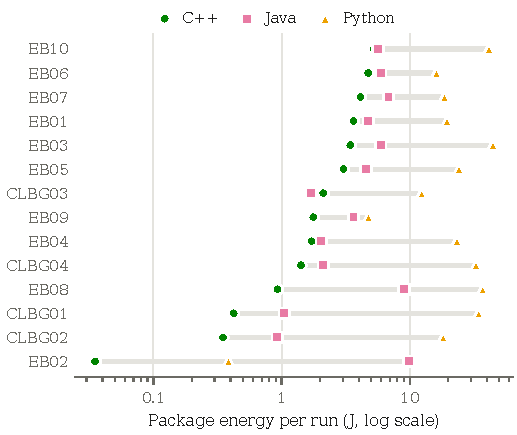
\includegraphics[width=\columnwidth]{laptop_languages}
  \caption{Median energy per run of generated programs (laptop).}
  \label{fig:languages}
\end{figure}

\begin{figure}[t]
  \centering
  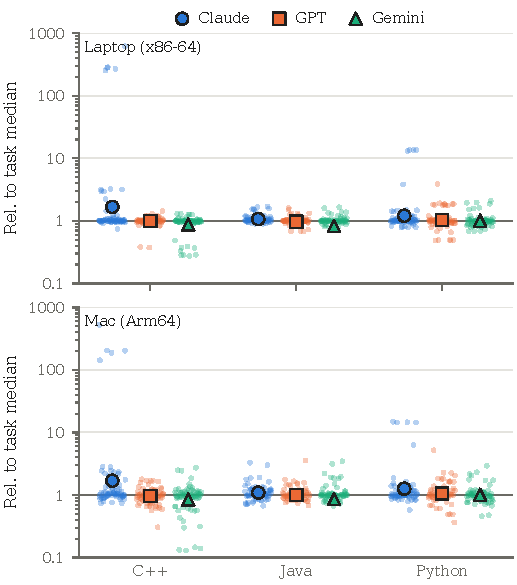
\includegraphics[width=\columnwidth]{llms}
  \caption{Program energy relative to its task--language median; large markers:
    geometric means.}
  \label{fig:llms}
\end{figure}

\begin{figure}[t]
  \centering
  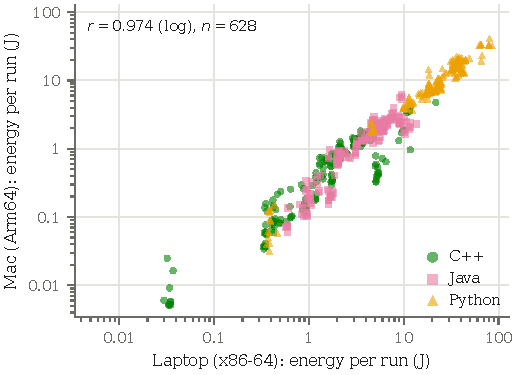
\includegraphics[width=\columnwidth]{platforms}
  \caption{Energy per program on laptop and Mac (different scopes).}
  \label{fig:platforms}
\end{figure}

% \section{Discussion}
\label{sec:discussion}

\TODO{Interpret results with respect to the RQs; relate to prior
work~\cite{solovyeva2025powerhungry,islam2025evaluating,apsan2025whereare,pereira2017energy};
analyse \emph{why} differences arise (e.g., algorithmic choices, library usage, data
structures) by qualitatively inspecting selected solutions; implications for developers
and for LLM benchmarking.}
  % merged/cut for the word limit (G6/G7)
\section{Threats to Validity}
\label{sec:threats}

RAPL, PMIC, and \texttt{powermetrics} (model estimates) capture
different scopes, so absolute values are not compared across platforms. The CLIs' hidden system prompts and differently calibrated effort levels make
\emph{LLM} a model--tool factor; models and CLIs evolve, so we record versions and dates.
All tasks are public and may be memorised. Solving an input repeatedly in one process
amortises one-time initialisation, and the 10\,s cap leaves some C++ runs below 0.1\,s,
where start-up weighs more. Results may not generalise to other models, languages, or
real-world code.

\section{Conclusion}
\label{sec:conclusion}

Language dominates the energy of LLM-generated code: Python needs about 13 times and Java
twice the energy of C++. The LLM matters less and mainly through algorithmic choices in a
few tasks; its ranking holds on x86 and Arm and across languages. As energy follows time,
runtime benchmarks remain a useful proxy. More platforms, open-weight models, and
energy-aware prompting are future work.


\FloatBarrier
\bibliographystyle{IEEEtran}
\bibliography{references}

\appendix
\section{Prompt Templates}
\label{app:prompts}

\Cref{fig:prompt-templates} shows both prompt templates verbatim; they are included directly
from the experiment repository (\texttt{experiment/prompts/}). Placeholders in braces are
filled per task and language: \texttt{\{language\}} is \emph{Python}, \emph{Java}, or
\emph{C++}; \texttt{\{language\_note\}} is given in \cref{tab:language-notes};
\texttt{\{problem\}} is the problem statement (EffiBench-X) or the task specification
(CLBG); \texttt{\{starter\}} is the EffiBench-X code skeleton for the respective language.
\Cref{fig:prompt-example} shows a fully rendered prompt.

\begin{table}[h]
  \centering
  \caption{Language-specific line \texttt{\{language\_note\}}.}
  \label{tab:language-notes}
  \footnotesize
  \begin{tabular}{@{}lp{0.72\columnwidth}@{}}
    \toprule
    Language & Text \\
    \midrule
    Python & Target Python 3.14 (CPython). \\
    Java   & Target Java 25 (OpenJDK). \newline
             \emph{Program template only:} The public class must be named \texttt{Main}. \\
    C++    & Target C++20. The code is compiled with \texttt{g++ -O2 -std=c++20}. \\
    \bottomrule
  \end{tabular}
\end{table}

\begin{figure*}[t]
  \textbf{\footnotesize (a) Function template (EffiBench-X tasks)}
  \VerbatimInput[fontsize=\scriptsize,frame=single,framesep=2mm]{../experiment/prompts/template_function.txt}
  \vspace{1ex}
  \textbf{\footnotesize (b) Program template (CLBG tasks)}
  \VerbatimInput[fontsize=\scriptsize,frame=single,framesep=2mm]{../experiment/prompts/template_program.txt}
  \caption{Prompt templates used for all LLMs.}
  \label{fig:prompt-templates}
\end{figure*}

\begin{figure*}[t]
  \VerbatimInput[fontsize=\scriptsize,frame=single,framesep=2mm]{../experiment/prompts/rendered/EB03/cpp.txt}
  \caption{Fully rendered prompt for task EB03 (Sum of Digit Differences of All Pairs) in C++.}
  \label{fig:prompt-example}
\end{figure*}


% Remove for the final version
\onecolumn
\listoftodos[Open TODOs]

\end{document}
